\chapter{La r\'ecuite simul\'e (chapitre 5 dans le cours heuristique)}

\section{Motivation}

En anglais: simulated anrealing. 
Propos\'e par Kirchkpatriche dans les ann\'ees 80.
Inspir\'e de la physique et plus de la m\'etallurgie.

\paragraph{Recuit :}
refroidissement lent d'un alliage m\'etallique conduisant \'a une structure cristalime qui est un minimum d'\'energie.

\paragraph{La trempe :} \'a l'oppos\'e du recuit on a le processus de termpage qui est refroidissement rapide ce qui donneune structure atomique qui est un min local 


$(\textcolor{red}{check- paper of 10/06/2015 page 3.2 } note 1)$ 

A haute temp\'erature on visite toutes les configurations de atomes (espace de recherche) et les configurations de basse \'en\'ergie restent plus longtemps car il faut assez d'energie pour en sortir.
Donc en basissant la temp\'erature, on va progrssivement trapper le syst\`eme dans les configuration d\'energie les plus basse.

\section{Principe de l'algorithme}
On cherche le min d'une fonction fitness not\'ee ici E pour \'energie

La proc\'edure est la m\^eme que discut\'e pr\'ecedemment 
\begin{itemize}
\item[\textbullet] On sp\'ecifie l'espace de retour
\item[\textbullet] le viosinage \'a travers des mouvement ou tranformation
\item[\textbullet] On d\'emarre avec une condition initale choisie au hazard (ou mieux )
\end{itemize}

A chaque i\'eration on g\'en\`ere un voisin en choisissant au hasarad une des transformation possible
Ce candidat est accept\'e comme point suivant selon la r\'egle dite de \underline{Metropolis}
	Soit $X_0$ la solution courante, d'\'energie $E_0$ est $E)1$
	et 
	Soit $X_1$ le candidat dont l\'energie 
	
	$X_1$ est accept\'e avec une probabilit\'e 
	$p=min(1,exp^{-(E_1 - E_0)/T})$
	ou $T$ est la "Temp\'erature de l'it\'eration courante 
	
$(\textcolor{red}{ Check--paper  3.2 note 2})$

si $\Delta E<0$, donc $E_1 < E_0$, alors $X_1$ a une \'energie meileur (au sens de plus petite) et sa probabili\'e d'acceptation est 1.

Mais si  $E_1 > E_0$ on a une prob. non-nulle de l'acceptation aussi.

Plus $\Delta E$ est grand ( plus on d\'egrade la fitness) plus la prob d'acceptation diminue (pour T donn\'e)]\\
Plus la temp\'erature 	est \'evalu\'ee plus on va  accepter des solution qui d\'egrade la fitness.

T grand : exploration (on accepte toutes solution)
T petite : exploration ( car on n'accepte que les am\'elioration)

En pratique la r\'egle de Metropolis est implement\'ee ainsi 
\begin{center}
rand(0,1) < $\exp^{-\Delta E / T}$ : acceptation \\
	sinon \hspace{2cm}rejet 
\end{center}

\subsection*{Organigramme}
$(\textcolor{red}{ Check paper 4 pour l'organigrame  note 2})$
$(\textcolor{red}{ Check exemple dans slide 72/341})$
\subsection*{Explication de l'exemple S74/341(important pour le TP):}
\begin{itemize}

\item on a la situation initial
\item additionner tt ces segement ( energie = longeur du chemin =f )(pr l'\'etat initiale)
\item dans la deuxieme phase on a un chemin moins compliqu\'e et on a paser de figure of T=0.1 a figure of  T=0.009 \\
	j'ai accepter chemin apres 20 acceptation de changement par exemple
	\item on baisse la temperature progressivemnet, on a 12 pali\'e  et progressiement minimiser la fitness 
	\item en tout y a eu 500 iteration 
	\item 20 palie de temperature 20*20=400 acceptation et tout le reste des 5000 c'est rejet
	\item si on part avec une temperature plus haut que  T=0.1 trop basse => j'arrive pas a plus soritir de certaines chemin \\
	donc il faut partir avec une temperature suffisement plus haut.
	\item si on change le taux d'acceptation de 300 ca prend plus du temps mais ca marche..

\end{itemize}
\subsection*{Explication de l'exemple S75/341(important pour le TP):}
\begin{itemize}

\item on a des emplacement possible qui sont les carret et sur chaque carrer on met une place et y a les ligne entre les 2 carre
\item les dfferente etape de recuit :\\on part avec T=25 et L=775 et on arrive a T=3 ...

\item revenant sur lexeple de 73 on a T=0.1 et dans S75 on a temperature T=25
alors ca affecte la fitness car dans la formule on a $\exp^{\Delta E/ T}$ et c'est le point significatifs
\end{itemize} 

\section{Convergence}

\textcolor{red}{Est ce que le recuit trouve l'optimum global  est \'a quelle condition ?}

Cette m\'etaheurisitique se pr\^ete \'a une analyse math\'ematique utilisant les cha\^ine de Markov\\ le r\'esultat de cette analuse donne le recuit 
\paragraph{\underline{Converge en porbabilit\'e :}} On peut obtenir une solution arbitrairement proche de l'optimum global avec une probabilit\'e arbitrairement proche de 1.\\ Pour que ce r\'esultat s'applique, il faut :
\begin{itemize}
\item les transfromation doivent \^etre r\'eversibles
\item Tout point de l'espace de recherche peut s'atteindre de tout autre en un nombre fini de transformation.
\item La temp\'erature initiale doit \^etre assez haute 
\item la tem\`erature doit d\'ecro\^itre assez lentement au cours des it\'erations:

\begin{center}
$T(t {\overbrace{iteration}}) =  \frac{C}{ log(t)}$ pour t grand \\

\end{center}
C est une constante qui d\'epend des variations d\'energie dans l'espace de recherche. Inconnue \`a priori:\\
Ce programme de temp. (temperature schedule)
est beaucoup trop lent pour une application pratique \\on pr\'ef\`ere une d\'ecroissance g\'eom\'etrique.
	
\end{itemize}

\subsection*{distribution de probabilit\'e }
On cherche la probabilit\'e que apr\'es $t$ it\'eration, on se trouve dans l'\'etat $X$ sachant qu'on est parti dans l'\'etat $y$ au temps $t=0$.\\
On aimerai que cette probabilit\'e soie telle que 
\begin{center}
\[ P(t->\infty,x)= \left\{
                \begin{array}{ll}
                  0 \ si\ x = xopt\\
                  1 \ sinon\\
                  
                \end{array}
              \right.
  \]
\end{center}

\paragraph{\underline{Notation:}} on note i et j des \'etats possible du recuit $ i \in S, j \in S $ \\

$P(t+1,j) = \sum{i} P(t,i)W_{ij}(t)$
o\`u $W_{ij}(t)$ est la probabilit\'e de passer de l\'etat i `a l'\'etat j \`a l'\it\'eration car la temp\'erature change avec les it\'erations.

\paragraph*{\underline{Distribution de probabilit\'e}}
Pour le r\'ecuit on peut sp\'ecifier la forme $W_{ij}$  \\
\[ W_{ij}(t)= \left\{
                \begin{array}{ll}
                  0 \ si\ j\ n'est\ pas\ voisin \ de \ i \\
                  \frac{1}{nombre voisins} \ P_mertopolis(E_i,E_j,T(t))\\
                   choix \  uniform \ parmi \ les \  voisins \ possible\  (pour\  le\  nombre \ de \ voisin)\\
                  
                  
                \end{array}
              \right.
  \]
et (prob de rejet) $W_{ij}(t) = 1-  \sum_{j\ voisins\ de\ i} W_{ij}(t) $\\
On a donc :
\begin{center}
$P(t,k) = \sum{i} P(t-1,i)W_{ik}(t-1)$ \\ 
= $\sum{[\sum{i} P(t-1,i)W_{ik}(t-1)]}$ \\
\textcolor{green}{check the rest on paper point 3}\\

\textcolor{red}{Suppososn maintenent que toutes les lignes de $ W(0,t-1) $ soit identiques donc  $ W(0,t-1)_{e_k} = W(0,t-1)_{1_k} $ }
\end{center}
Dans ce cas, $W(0,t-1)_{1_k}$ ne d\'epend plus de l et peut \^etre de la somme:
\begin{center}
$P(t,k) = W(0,t-1)_{1_k}\sum_{e}P(0,e)$  \\ avec $\sum_{e}P(0,e)$ =1 car on choisit formcement 1 \'etat initial \\ 
$=> P(t,h) = W(0,t-1)_{1_k}$ \\


Donc la prob d'\'ete dans l'\'etat k au temps t devient independant de l'\'etat intial 
\end{center}

La propri\'et'e que\\
$W(0,t-1)_{1_k}$    est identique pour tout e est vrai si :\\
$t -> \infty $\\
$T_0 est assez grand$
De plus si la decroissance de T est assez lente  \\
$P(t,k) = W(0,t-1)_{1_k}$ va \^etre un pour l'opt globale et z\'ero sinon

\textcolor{yellow}{end of session of 10/05/2015}\\
\noindent\rule{12cm}{0.4pt}

\newpage
\LARGE Lecture of 12/ oct / 2015
\hfill Missed Lecture
\newpage


\centerline{Chapitre 3 Lecture of 19/ oct / 2015}
\section{La piste des phéromones : une optimisation
naturelle}

\subsection{Deuxieme experience }
\textcolor{red}{check the graph on  page 30 of heuritique doc}
les deux dernier sont empruntés mais au cours ... COPY THE RESTE FROM SOMEONE

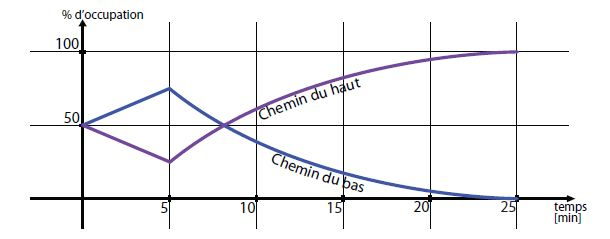
\includegraphics[scale=0.9]{./images/resultatexperimental.jpg}

\section{Methode de probabilité}

copy the reste from ...

On va supporser que $P_u(n+1)$ dépend des phéromones laissées par les n fourmis qui ont passés avant.
On définit 

\subsection{L'algorithme AS}

Procédure \\
> A chaque it\'eration t on lance les m fourmis \`a travaers les n villes\\
> Chacune de ces m fourmis ex\'ecute un parcours du TSP\\
> Consid\'erons le cas de la fourmi n k (k=1,...m) qui \'a l'it\'eration t se trouve \'a la ville i et doit choisir les prochaine ville j o\`u aller.\\
> Dans l'algo AS, la ville j est choisie aucc prob $P_{ij}$ 
\begin{center}
$$ P(t->\infty,x)= \left\{
                \begin{array}{ll}
                  0 \ si j \notin J \\
                  \frac{t_{ij}(t-1)]^\alpha [\eta_{ij}]^\beta}{\displaystyle\sum_{\ell\in J} [(t-1)][\eta{i\ell}]}\\
                \end{array}
              \right.
  $$
\end{center}





